\documentclass{ieeeaccess}

% Custom packages
\usepackage{caption}
\usepackage{subcaption}
\usepackage{hyperref}
\usepackage[nolist, printonlyused]{acronym}

% Template packages
\usepackage{cite}
\usepackage{amsmath,amssymb,amsfonts}
\usepackage{algorithmic}
\usepackage{graphicx}
\usepackage{textcomp}

\def\BibTeX{{\rm B\kern-.05em{\sc i\kern-.025em b}\kern-.08em
    T\kern-.1667em\lower.7ex\hbox{E}\kern-.125emX}}

\begin{document}
    \begin{acronym}
    \acro{REG}[REG]{renewable energy generator}
    \acro{ESS}[ESS]{energy storage system}
    \acro{BESS}[BESS]{battery energy storage system}
    \acro{PV}[PV]{photovoltaic}
    \acro{EMS}[EMS]{energy management system}
    \acro{DER}[DER]{distributed energy resource}
    \acro{EOL}[EOL]{end of life}
    \acro{SOC}[SoC]{state of charge}
    \acro{SOH}[SoH]{state of health}
    \acro{DOD}[DoD]{depth of discharge}
    \acro{BMS}[BMS]{battery management system}
    \acro{RUL}[RUL]{remaining useful life}
    \acro{EM}[EM]{electrochemical model}
    \acro{ECM}[ECM]{equivalent circuit model}
    \acro{MILP}[MILP]{mixed integer linear programming}

    \acro{LIB}[LIB]{lithium-ion battery}
    \acroplural{LIB}[LIBs]{lithium-ion batteries}

    \acro{MG}[MG]{microgrid}
    \acroindefinite{MG}{a}{an}
\end{acronym}

    \history{Date of publication xxxx 00, 0000, date of current version xxxx 00, 0000.}
    \doi{10.1109/ACCESS.2017.DOI}

    \title{A Novel Battery Wear Model For Energy Management In Microgrids}

    \author{
    	\uppercase{Lucas B. Rhode}\authorrefmark{1},
    	\uppercase{Adriano B. de Almeida}\authorrefmark{2}
    	\uppercase{and Marcos A. Izumida}\authorrefmark{3}
    }
    \address[1]{Sustainable Energies Center, CERTI Foundation, Brazil (e-mail: lrh@certi.org.br)}
    \address[2]{Western Parana State University, Brazil (e-mail: adriano.almeida@unioeste.br)}
    \address[3]{Sustainable Energies Center, CERTI Foundation, Brazil (e-mail: mlz@certi.org.br)}

    \markboth
    {Author \headeretal: Preparation of Papers for IEEE TRANSACTIONS and JOURNALS}
    {Author \headeretal: Preparation of Papers for IEEE TRANSACTIONS and JOURNALS}

    \corresp{Corresponding author: Lucas B. Rhode (e-mail: lrh@certi.org.br)}

    \begin{abstract}
        This paper proposes a novel battery wear model for \ac{MG} energy management applications. This model is based on a popular battery wear model originally proposed for vehicle-to-grid (V2G) applications. The presented model can be easily parameterized to fit the cycle life data of almost any battery and yields the wear cost of a charge/discharge event as function of the variation in the state of charge (SOC) of the battery. This wear model is incorporated into an energy management algorithm to optimize the operation of a grid-connected MG using a day-ahead planning strategy. To test the model, four simulated scenarios are considered in an MG composed of a diesel generator, a photovoltaic (PV) system, a residential load and, naturally, a battery storage system (BESS). The inclusion of the battery wear model leads the optimizer to be more selective about battery usage, cycling the battery at SOC levels that minimized battery wear, effectively prolonging its lifespan.
    \end{abstract}

    \begin{keywords}
        battery management systems, energy storage, energy management, microgrids
    \end{keywords}

    \titlepgskip=-15pt

    \maketitle

    \section{Introduction}
    \label{sec:introduction}
    \PARstart{E}{lectricity} has become an essential element for society in the last century. With growing energy consumption aggravating the rise in CO\textsubscript{2} emissions, achieving full sustainability is one of the greatest challenges of our modern society. As part of this effort, grid operators are continually deploying new \acp{REG}, such as in wind farms and \ac{PV} power stations, supplying a record high of more than 11\% of the world's electricity in 2020 \cite{EMBER2021}.

    In \acp{MG}, \acp{REG} play a vital role and, as such, \acp{ESS} are one of the main components in these environments. While traditional sources can store energy in fuels tanks, water reservoirs and kinetic energy, most renewable sources need external devices to store their output when it is abundant, to later return it to the grid \cite{STECCA2020}. Additionally, with combined renewable generation and energy storage, \iac{MG} can coordinate resources to achieve increased system efficiency by reducing generation-demand mismatches, using techniques such as time-shifting, peak shaving and valley filling \cite{WANG20196201, LI2020106058, PARRA2015576, ZHANG2019772}.

    There are many different technologies for storing energy, such as pumped hydros, fuel cells, flywheels, supercapacitors and others \cite{IBRAHIM2008}. However, \acp{BESS} are commonly the preferred choice for energy management applications. They present good energy density, scalability, efficiency and technical maturity that makes them a good fit for energy storage in small-scale systems \cite{KOCER2019, martins2018optimal, FU20136749070}.

    Among the available technologies, \acp{LIB} and lead-acid are predominant in modern \ac{BESS} applications \cite{FU20136749070, ALSAIDAN8094981}. Historically, lead-acid batteries were preferred for their lower upfront cost, in spite of lithium cells having a greater overall performance and longevity \cite{wang2013li, xu2010lithium}. Recently, the growing interest in electric vehicles and its associated mass production have significantly reduced the cost of this technology, making it the most popular energy storage method in \acp{MG} \cite{mongird20202020, BBERG2020, zhang2018energy}.

    Still, \acp{BESS} are costly, which becomes even more evident when its useful life is taken into account. Batteries have a limited number of achievable discharge and recharge cycles before they reach their \ac{EOL}, at which point the cells no longer meet minimal criteria for the intended application \cite{ZHU2021100537, hart2014modeling}.

    The \ac{EOL} can be defined as a reduction of 20\% to 30\% of the battery's \ac{SOH} in general applications \cite{ECKER2014, NARAYAN2018}. In more sensitive environments where performance of the \ac{ESS} is crucial, more specific criteria may apply \cite{WOOD20115147, JACOB2020101565}. To determine the \ac{SOH}, \acp{BMS} employ various methods and, although there is no fixed definition for \ac{SOH}, many references utilize the effective capacity to evaluate it and estimate the \ac{RUL} of a battery \cite{TIAN2020120813, rezvanizaniani2014review, BIOLOGIC2021, bose2002battery}.

    \ac{SOH} estimation models can be further divided into experiment-based and model-based approaches. Experimental models are attractive for being simpler in terms of computational complexity, however it requires a large number of experiments to assess how the variables change as cells age \cite{XIONG2018264}. In \cite{li2019lithium, kang2014new} machine learning and big Data are use as modern approaches to predict battery behavior based on experimental results, however the literature still lacks the necessary amount of data volume and diversity to correctly train models that work with batteries of different compositions, size and manufacturers \cite{maheshwari2020optimizing}.

    The acquisition of experimental data for each specific \ac{BESS} can be unrealistic in practical cases. Usually the \ac{MG} operator does not have the time, technical or financial resources to execute such tests. To overcome this, model-based methods can be applied.

    \acp{EM} present a highly adaptive approach to achieve highly accurate wear estimation, as demonstrated in \cite{XIONG2018264}. These models can be applied in dedicated \acp{BMS} that need to provide an indication of remaining capacity, \ac{RUL} and current \ac{SOH}. In such scenarios, the processing power of the local controller can be dedicated entirely to data acquisition and online calculation of these performance indicators.

    \ac{ECM} offer a practical way to model both the static and dynamic behavior of cells for battery management in local controllers. This approach is useful since it can be parameterized and implemented to estimate multiple indicators such as \ac{SOC}, \ac{SOH} and power capability \cite{verbrugge2004adaptive, verbrugge2007adaptive}. However, it still demand a great knowledge of battery parameters and their relationship with each other and external conditions, such as temperature and operational history \cite{zhang2018online}.

    These approaches can certainly be made highly accurate with increased model complexity and data availability. However, in centralized \acp{EMS} the additional communication requirements for acquiring and processing all the necessary data can limit the applicability of these models \cite{DIMEASHATZIARGYRIOU2005}.

    As such, this paper proposes a novel linearized model that blends both model and experimental-based approaches that require only simple \ac{ACC} curves that can be obtained relatively easily from datasheets or manufacturers and resellers. The goal of this formulation is to provide a simple wear cost quantifier that can be used to orientate the \ac{EMS} of \iac{MG} as to whether or not use the \ac{BESS} in detriment of other strategies -- such as dispatching diesel generators or purchasing power from the utility grid -- rather then providing a highly accurate battery state predictor.

    We base our modified wear cost model on \cite{HAN2014} and add (i) a generic formulation, from which operators can derive their own customized models; (ii) a concrete implementation of that formulation that can be parameterized to fit lead-acid and \ac{LIB} aging curves; (iii) a linearization of this implementation that can be directly applied into \ac{MILP} solvers.

\section{Battery Wear Formulation}

    In power applications the two main variables affected by battery aging is (i) effective storage capacity and (ii) maximum power output \cite{han2014comparative, chemali2015minimizing, al2010mathematical}. The underlying mechanisms that cause these symptoms are multiple and complex, involving chemical reactions that depend on battery composition, storage conditions and operation - mainly temperature, charge/discharge rate (C-rate), \ac{SOC} and \ac{DOD} \cite{xiong2020lithium, vetter2005ageing, calearo2019modeling}.

    While in batteries used for automotive and frequency regulation purposes high instant power is usually an important requirement, in peak-shaving and PV-BESS applications storage capacity is usually a bigger concern. Studies \cite{hesse2017lithium, sufyan2019optimal, asano2007methodology} indicate that for these applications, lower power-to-energy ratios are preferred and batteries are usually operated for a few hours under 1C rates. From this, it can be assumed that the impact of \ac{SOC}, \ac{DOD} and temperature are far more relevant for degradation models used in \acp{EMS}.



%    The battery lifetime published by manufactures usually assumes that the battery is fully
%charged and discharged each cycle at an ideal ambient temperature
%

%    usou custo fixo R$/kWh para desgaste: https://www.sciencedirect.com/science/article/pii/S0378779616304692



    The wear cost quantification is based on the concept of a wear density function $w(s)$. It takes as argument the SOC of the battery ($s$) and returns a marginal cost in monetary units per battery percentage. Then, a charging/discharging event starting at the initial SOC $s_{0}$ and ending at $s_{f}$ could have its associated wear cost $C_{b}$ evaluated through the following integral:
    \begin{equation}
        C_{B}(s_{0}, s_{f}) = \int_{s_{l}}^{s_{u}}w(s)ds
        \label{eq:Cb(s0,sf)}
    \end{equation}
    where $s_{l}$ and $s_{u}$ are the lower and upper SOC boundaries of the charging/discharging event, formally: $s_{l} = min\{s_{0}, s_{f}\}$ and $s_{u} = max\{s_{0}, s_{f}\}$. As such, the value of the definite integral is always positive if $w(s)$ is positive.

    Therefore, by solving this integral we will be able to find a closed-form expression to calculate the wear cost of a single charge or discharge event using only two inputs: starting and final SOC.

    \subsection{Battery cycle life}
    Lithium-ion batteries do not suffer from ``sudden-death'' failure. Instead they exhibit a gradual decrease in performance over their service life. The end of life might be defined as a reduction in capacity (typically 20 to 30\%) or an increase in internal resistance, which may be particularly important in power applications. For example, in \cite{ECKER2014} it is characterized either by battery capacity falling under 70\% of the original or when its internal resistance triples; in \cite{NARAYAN2018} the thresholds are 80\% of the original capacity or 80\% of the state of health, an indicator of overall battery performance.

    Most manufacturers inform battery life in terms of achievable cycle count, that is, the number of charge/discharge events that a battery support before becoming unsuitable for a given application. In this context, each cycle is composed by a discharge, beginning at 100\%, followed by a recharge until 100\%. As illustrated in Fig. \ref{fig:acc_curves1}, batteries have cycle lives that decay exponentially with higher DOD levels.

    \begin{figure}[htbp]
        \centering
        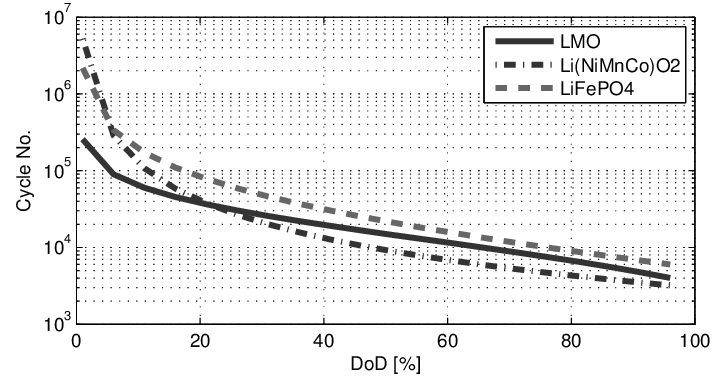
\includegraphics[width=0.35\textwidth]{figures/acc_curves1.png}
        \caption{Typical cycle life of lithium-ion batteries as function of DOD \cite{XU2016}.}
        \label{fig:acc_curves1}
    \end{figure}

    Note that DOD is defined as the difference between the initial and final SOC, being positive for discharging and negative for recharging. In this formulation it will be represented by $d$:
    \begin{equation}
        d = s_{0}-s_{f}
        \label{eq:dod(s)}
    \end{equation}

    Since life cycle information is usually given at discrete DOD levels, it is useful to interpolate those data points. For that, let us define a generic function $ACC(d)$ to represent the achievable cycle count in function of the DOD. This function may have any format in order to better fit different battery chemistries.

    \subsection{Cost per half cycle --- starting at 100\% SOC}
    Given that $ACC(d)$, independent of its form, yields the number of times that a battery can be cycled, it is logical to assume that if we divide the price of the battery by $ACC(d)$, the result would be the cost associated with one full cycle. Then, to assess the cost of a single half cycle (i.e. either the charging or discharging part of a cycle), this value should further be divided by two, thus:
    \begin{equation}
        \mathrm{Cost \; per \; half \; cycle} = \frac{B_{P}}{2 \cdot ACC(|d|)}
        \label{eq:costPerHalfCycle1}
    \end{equation}
    where $B_{P}$ is the battery price and the modulus operator is used to make the expression valid both charging and discharging processes.

    That is, if a half cycle either starts or ends at 100\% SOC, the DOD could be plugged into \eqref{eq:costPerHalfCycle1} and the expression would yield the wear cost associated with that event.

    Therefore, by definition, equation \eqref{eq:costPerHalfCycle1} is a solution to the cost function $C_{B}(s_{0}, s_{f})$ at a specific range, either for charging events, $C_{B}(s_{0}, 1)$, or a discharging events $C_{B}(1, s_{f})$. However, for ranges that neither start or end at 100\% SOC, another expression must be derived.

    \subsection{Cost per half cycle --- any range}

    For charging, we can replace $d=s_{0}-1$ in \eqref{eq:costPerHalfCycle1} and equate it to \eqref{eq:Cb(s0,sf)}, resulting in:
    \begin{equation}
        \int_{s_{0}}^{1}w(s)ds = \frac{B_{P}}{2 \cdot ACC(|s_{0}-1|)}
        \label{eq:costCharging100}
    \end{equation}
    where $s_{0}$ is the lower limit of integration because it will always be less or equal to 1 (there are no SOC levels greater than 100\%).

    Expanding the integral on the left hand side of \eqref{eq:costCharging100}:
    \begin{equation}
        W(1) - W(s_{0}) = \frac{B_{P}}{2 \cdot ACC(|s_{0}-1|)}
        \label{eq:fundamentalTheorem1}
    \end{equation}
    where $W(s)$ is a primitive of $w(s)$.

    A similar expression can be obtained for the discharging event, when $d=1-s_{f}$, yielding:
    \begin{equation}
        W(1) - W(s_{f}) = \frac{B_{P}}{2 \cdot ACC(|1-s_{f}|)}
        \label{eq:fundamentalTheorem2}
    \end{equation}

    By subtracting \eqref{eq:fundamentalTheorem2} from \eqref{eq:fundamentalTheorem1} and rewriting in compact integral notation, we arrive at a partial solution to \eqref{eq:Cb(s0,sf)}:
    \begin{equation}
        \begin{aligned}
            \int_{s_{0}}^{s_{f}}w(s)ds = & \frac{B_{P}}{2 \cdot ACC(|s_{0}-1|)}            \\
            & \;\;\;\; - \frac{B_{P}}{2 \cdot ACC(|1-s_{f}|)}
        \end{aligned}
        \label{eq:partialSolution}
    \end{equation}

    This expression is only valid for $s_{0} \le s_{f}$, that is, for recharging. The process can be repeated for the case where $s_{0} > s_{f}$ and the result would be \eqref{eq:partialSolution} with a flipped sign. Instead, a single closed-form equation can be summarized using the modulus operator. The result is the solution to the cost function $C_{B}(s_{0}, s_{f})$ defined in \eqref{eq:Cb(s0,sf)}:
    \begin{equation}
        C_{B}(s_{0}, s_{f}) = \frac{B_{P}}{2} \left| \frac{1}{ACC(1-s_{f})} - \frac{1}{ACC(1-s_{0})} \right|
        \label{eq:finalSolution}
    \end{equation}
    where, since both $s_{0}$ and $s_{f}$ are always less or equal to one, the inner modulus operator was dropped.

    The model proposed in \eqref{eq:finalSolution} is valid through the entire SOC range, 0\% to 100\%, as long as $1/ACC(s)$ is continuous in that same range and, since it does not assume any particular format for the $ACC(d)$, it also is fairly independent of battery chemistry.

    This result adds two levels of abstraction to \cite{HAN2014} because it accepts almost any generic form of $ACC(d)$ without the need to derive a new model. It also uses only the initial and final SOC of each half cycle, therefore there's no need to know the power flow of the battery at each instant, only the amount of energy needed. This provides a more convenient way to calculate costs in energy management systems (EMS).

    \subsection{Curve Fitting Model}
    As for the cycle life curve $ACC(d)$, the model used in \cite{HAN2014} is the reciprocal function: $ACC(d) = a_{0} \cdot d^{-a_{1}}$, where $a_{0}$ and $a_{1}$ are coefficients of the nonlinear regression. This provides a good fit for the cycle life curve of some specific batteries, especially lead-acid ones, but leaves room for improvement to better fit other chemistries.

    We were able to explore other formats, such as exponential $ACC(d) = a_0 \mathrm{e}^{-a_1 d}$ and logarithmic $ACC(d) = a_0 - a_1 \ln(d)$, and, although these elementary functions performed well on specific batteries, they failed to provide a universal model. Based on empirical data, we found that a more generic result could be obtained by combining the reciprocal function and exponential function:
    \begin{equation}
        ACC(d) = a_0 \cdot d^{-a_1} \cdot \mathrm{e}^{-a_2 d}
        \label{eq:ACC(d)}
    \end{equation}
    where $a_0$, $a_1$ and $a_2$ are coefficients that can be obtained by methods such as the least squares fitting.

    Equation \eqref{eq:ACC(d)} proved to be a good empirical model to fit the cycle life curves of different commercial battery chemistries and manufacturers, as shown in Fig. \ref{fig:acc(d)}. Therefore, this was the format chosen to be implemented in this study.
    \begin{figure}[!h]
        \begin{subfigure}{.235\textwidth}
            \centering
            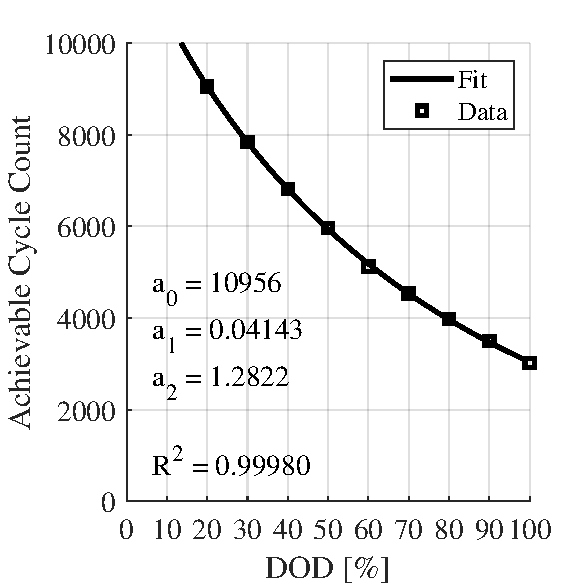
\includegraphics[width=\linewidth]{figures/acc_fitting_NeoVolta_NV24_LiFePO4.pdf}
            \caption{NeoVolta NV14 (LiFePO4)}
            \label{fig:accNeovolta}
        \end{subfigure}
        \begin{subfigure}{.235\textwidth}
            \centering
            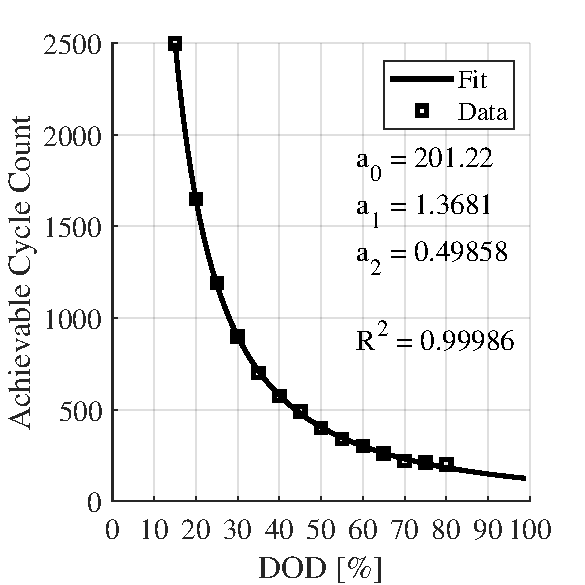
\includegraphics[width=\linewidth]{figures/acc_fitting_Moura_12MF220_lead-acid.pdf}
            \caption{Moura 12MF220 (lead-acid)}
            \label{fig:accMoura}
        \end{subfigure}

        \begin{subfigure}{.235\textwidth}
            \centering
            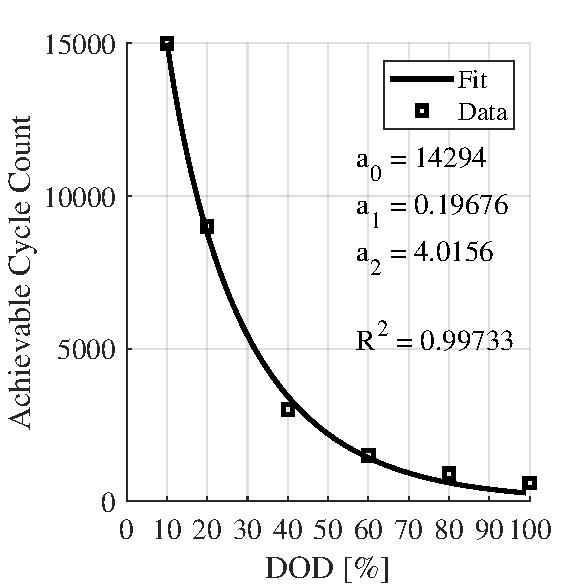
\includegraphics[width=.8\linewidth]{figures/acc_fitting_Unknown_model_LiPO4.pdf}
            \caption{Generic model (LiFePO4) \cite{BATUNI2020}}
            \label{fig:accLipeo4}
        \end{subfigure}
        \begin{subfigure}{.235\textwidth}
            \centering
            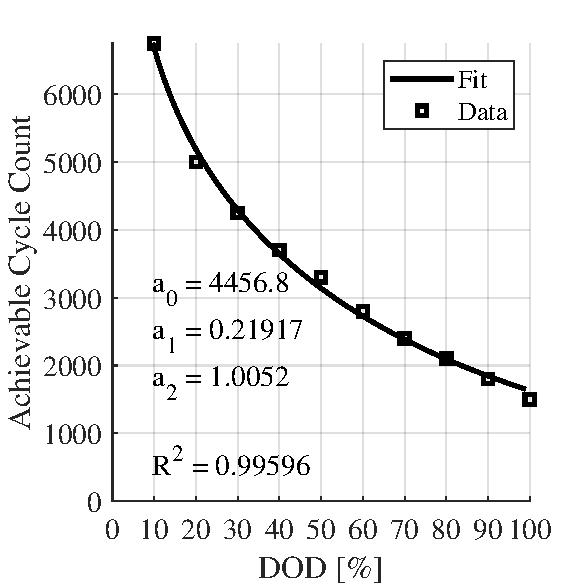
\includegraphics[width=.8\linewidth]{figures/acc_fitting_Rolls_16CH35P_lead-acid.pdf}
            \caption{Rolls 8 CH 33P (lead-acid)}
            \label{fig:accNimh}
        \end{subfigure}
        \caption{Equation \eqref{eq:ACC(d)} fitted to data from different battery models.}
        \label{fig:acc(d)}
    \end{figure}

    \subsection{Normalized Wear Density Function}
    By taking the partial derivative of \eqref{eq:partialSolution} with respect to $s=s_f$ and dividing it by the capacity $M$ of the battery, we arrive at the normalized wear density function:
    \begin{equation}
        w_n(s) = \frac{w(s)}{M} = - \frac{B_P}{2M} \cdot \frac{d}{ds} \left( \frac{1}{ACC(1-s)} \right)
        \label{eq:wn(s)}
    \end{equation}

    By substituting \eqref{eq:ACC(d)} in \eqref{eq:wn(s)} and considering $s \le 1$, the normalized wear density function becomes:
    \begin{equation}
        w_n(s) = \frac{B_P}{2M} \cdot \frac{a_1(1-s)^{a_1-1} + a_2(1-s)^{a_1}}{a_0} \cdot \mathrm{e}^{a_2(1-s)}
        \label{eq:wn(s)a0a1a2}
    \end{equation}

    Although the expression in \eqref{eq:finalSolution} yields the wear cost of cycling the battery, it provides little insight on how the SOC level impacts the cycle life of a battery. For qualitative analysis, the density function such as \eqref{eq:wn(s)a0a1a2}, provides a tool to evaluate the performance of the battery across multiple SOC ranges. Moreover, the average value of the wear density function is also useful when evaluating the overall cost-benefit of different battery models, as it can differentiate batteries not only by price and capacity, but also by durability. The average value of \eqref{eq:wn(s)a0a1a2} is calculated as:
    \begin{equation}
        \overline{w_n} = \frac{B_P}{2M} \frac{\mathrm{e}^{a_2}}{a_0}
    \end{equation}

    \section{Energy Management Model}
    To test the battery wear model, we modified the energy management algorithm proposed by \cite{SANTOS2018}, which initially used a fixed cost per kilowatt-hour to evaluate the cost of using the BESS. The model implements a day-ahead planning strategy using mixed integer nonlinear programming (MINLP) that aims to minimize the operational cost of an MG composed by a diesel generator, BESS, PV system and a load, as shown in Fig. \ref{fig:mg1}.
    \begin{figure}[htbp]
        \centering
        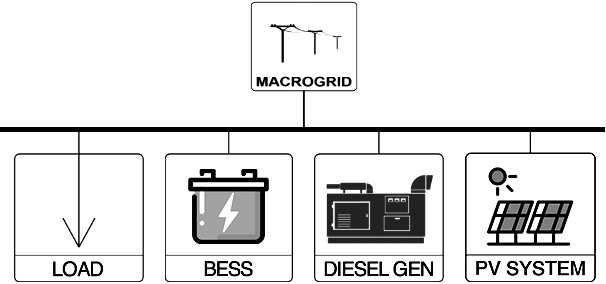
\includegraphics[width=0.4\textwidth]{figures/mg2.png}
        \caption{Diagram of the simulated MG.}
        \label{fig:mg1}
    \end{figure}

    The objective of the day-ahead planning is to calculate setpoints that all DERs within the MG should follow in order to supply the load with the lowest operational cost possible. This may lead to strategies such as charging batteries in off-peak hours, with cheap energy, and use that to minimize energy purchase during peak-hours. Therefore the importance of having a model to quantify battery wear.

    The MG is modeled as a single-bus system and, as such, no distribution line losses are considered. The model also does not account for the dynamic behavior of the DERs, as this is attribution of real-time management systems. The day-ahead planning is based on predictions of load profiles and solar generation profiles for the following 24 hours. It considers two electricity tariff levels, for peak and off-peak hours, and two contracted demands, also for peak and off-peak hours. Reverse power-flow (MG exporting power to the utility grid) is rewarded with a feed-in tariff that is a fraction of the energy purchase tariff.

    The model uses a discrete-time approach with finer timesteps for the first hour and larger timestemps for the remaining 23 hours. This ensures higher time-definition for the near-future, where demand and generation forecasts are more precise, but limits computational burden of the optimization process. This is important because day-ahead planning strategies usually update their setpoints every few minutes as real load and generation profiles naturally deviate from predictions, which places a time constraint in solving the optimization problem.

    \subsection{Objective Function}
    The objective function that defines the optimization problem of this study is the sum of operational costs and energy purchase expenses at each discretization interval:
    \begin{equation}
        Z = \sum_{t=1}^T(Z_{IO}[t] + Z_D[t] + Z_B[t] + Z_P[t])
        \label{eq:z1}
    \end{equation}
    where:
    \begin{itemize}
        \item $Z$: total operational cost over the simulation period;
        \item $t$: time-discretization index (1, 2, 3...);
        \item $T$: discretization interval count;
        \item $Z_{IO}$: energy import cost ($+$) or export revenue ($-$);
        \item $Z_{D}$: operational cost of the diesel generator;
        \item $Z_{B}$: battery wear cost; and
        \item $Z_{P}$: penalty for exceeding maximum contracted demand.
    \end{itemize}

    Notice that there is no term associated with PV system power output because its operational cost is usually independent of energy delivery.

    \textbf{Energy import cost and export revenue} --- modeled with a feed-in tariff:
    \begin{equation}
        Z_{IO}[t] = \left( \mu_i[t] \cdot P_i[t] - \mu_e[t] \cdot P_e[t] \right) \cdot dt[t]
    \end{equation}
    where $\mu_i[t]$ and $\mu_e[t]$ are the purchase and feed-in tariffs parameters, respectively; $P_{i}[t]$ and $P_{e}[t]$ are the power import and export variables, respectively; and $dt[t]$ is the size of the discretization interval parameter. Note that power imported at a rate under the contracted limit is calculated separately from the power imported above the contracted limit, that is, $P_i[t]$ is always lower then the contracted demand.

    \textbf{Diesel fuel cost} --- the cost of diesel fuel, modeled using a quadratic model and a startup cost:
    \begin{equation}
        Z_D[t] = \mu_d \cdot (a^{}_d P_d[t]^{2} + b_dP_d[t] + c_d) \cdot dt[t] + S_d[t]
    \end{equation}
    where $\mu_d$ is the parameter for diesel cost per liter; $a_d$, $b_d$ and $c_d$ are the consumption parameters of the diesel generator; $P_d[t]$ is the power output variable of the diesel generator; and $S_d[t]$ is the startup cost variable of the generator at each discretization interval, which is zero if the generator has been started at a previous interval or if the power output is zero. The power output of the diesel generator is also subject to minimum and maximum limits.

    \textbf{Maximum demand penalty} --- modeled using a very high tariff for power import:
    \begin{equation}
        Z_P[t] = \mu_{pi}[t] \cdot P_{pi}[t] \cdot dt[t]
    \end{equation}
    where $\mu_{pi}[t]$ is the parameter that defines the tariff for buying power at a rate above the contracted limit, usually several times higher then $\mu_i[t]$; and $P_{pi}[t]$ is the variable for importing power above the contracted limit, which is only greater then zero when $P_i[t]$ has reached the contracted demand limit.

    \textbf{Battery wear cost} --- obtained by substituting \eqref{eq:ACC(d)} in \eqref{eq:finalSolution}, where the initial and final SOC, $s_0$ and $s_f$, become $s[t-1]$ and $s[t]$, respectively:
    \begin{equation}
        \begin{aligned}
            C_b[t] & = \frac{B_P}{2a_0} \Bigg|(1-s[t])^{a_1}\mathrm{e}^{a_2(1-s[t])} \\
            & - (1-s[t-1])^{a_1}\mathrm{e}^{a_2(1-s[t-1])} \Bigg|
        \end{aligned}
    \end{equation}

    In order to realize the power balance of the MG, power output of the battery is calculated by converting battery percentage to energy transfer rate, i.e. $P_b[t] = \frac{M(s[t]-s[t-1])}{dt[t]}$, which is negative for battery recharge.

    The complete MINLP model is available on the GitHub repository \href{https://github.com/lucasrhode95/adams}{github.com/lucasrhode95/adams}, where we also made available an application for day-ahead planning simulations.

    \section{Methodology \& Simulations}
    Parameters for the simulations were based on commercially available products and average electricity rates in the United States. The diesel generator parameters are from Caterpillar's DE22E3 22 kVA model; the residential load profile was borrowed from the U.S. Department of Energy public database \cite{DOE2013}, scaled to achieve a consumption of 300 kWh/day; and the PV generation is a generic autumn profile, delivering 100 kWh/day. The net load profile (load minus PV generation) is shown in Fig. \ref{fig:net-load}, where it can be seen that the PV generation exceeds demand from 10 a.m. to 14 a.m.
    \begin{figure}[htbp]
        \centering
        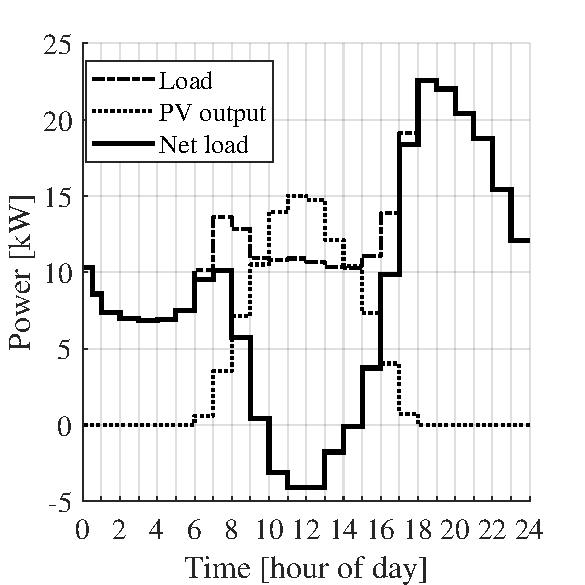
\includegraphics[width=0.3\textwidth]{figures/net_load.pdf}
        \caption{Profiles for residential load, PV generation and the resulting net load used.}
        \label{fig:net-load}
    \end{figure}

    For batteries, two commercially available options were considered: NeoVolta's NV14 (14.4 kWh) and Rolls' 8 CH 33P (7.12 kWh), hereafter referred as BESS A and BESS B, respectively.

    The cycle life curve of both systems were shown in Fig. \ref{fig:acc_curves1}, while the wear density of both is shown in Fig. \ref{fig:wn_curves1}, where the lowest wear density points are highlighted: 0.088123 USD/kWh at 87\% SOC for BESS A, and 0.18287 USD/kWh at 75\% SOC for BESS B. It also can be observed that wear density increases at both ends of the SOC, an expected result given that both very low and very high SOC levels are known to reduce battery life \cite{ECKER2014, WIKNER2018}.
    \begin{figure}[!h]
        \begin{subfigure}{.235\textwidth}
            \centering
            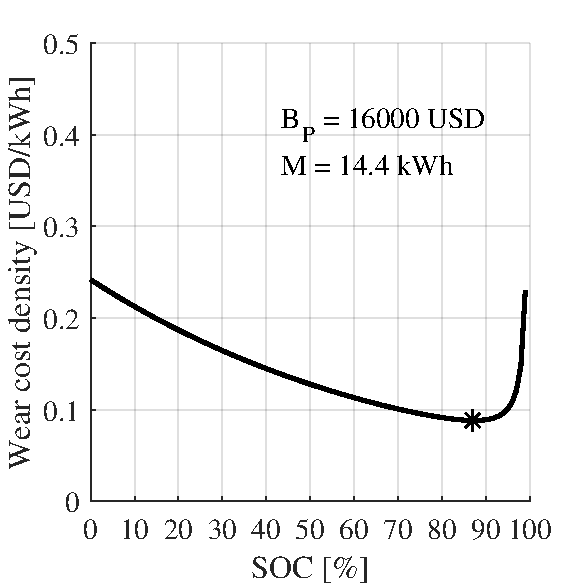
\includegraphics[width=\linewidth]{figures/marginal_NeoVolta_NV24_LiFePO4.pdf}
            \caption{BESS A (LiFePO4)}
            \label{fig:wn_curves1A}
        \end{subfigure}
        \begin{subfigure}{.235\textwidth}
            \centering
            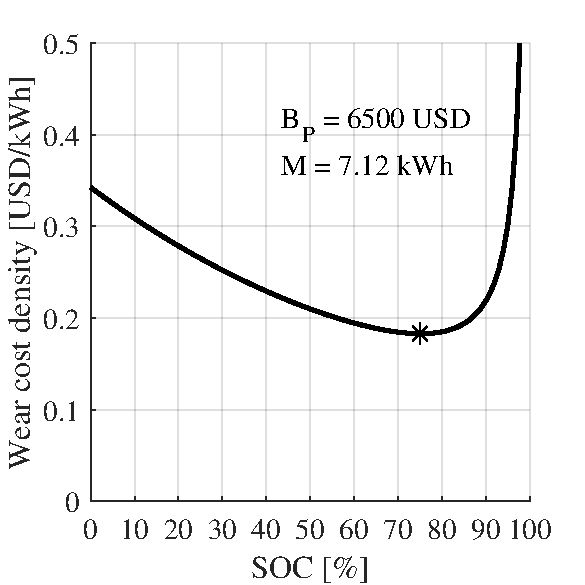
\includegraphics[width=\linewidth]{figures/marginal_Rolls_8CH33P_lead-acid.pdf}
            \caption{BESS B (lead-acid)}
            \label{fig:wn_curves1B}
        \end{subfigure}
        \caption{Wear density function \eqref{eq:wn(s)a0a1a2} of both batteries.}
        \label{fig:wn_curves1}
    \end{figure}

    For the tests, both systems were considered to have an efficiency of 94\%, a self discharge rate of 0.2 \%/hour and charge/discharge rate was limited to 0.5C.

    As for the electricity tariffs, off-peak prices were set at 0.1048 USD/kWh and peak prices at 0.2096 USD/kWh. Feed-in tariff was set at 0.035 USD/kWh for peak and off-peak hours. The contracted demand at was defined as 23 kW and 18.4 kW for off-peak and peak-hours, respectively. Above these limits, tariffs were defined as 10 USD/kWh for off-peak hours and 20 USD/kWh for peak-hours.

    In order to keep both systems with roughly the same capacity, we considered that BESS B is composed of two batteries, therefore doubling its cost and capacity to 13,000 USD and 14.24 kWh, respectively.

    In addition, the SOC of both systems were set to start and end at 50\%, so that all energy usage must be replenished before the end of the day, plus losses.

    \subsection{Results}
    There were four scenarios analyzed with varying composition of BESS models and diesel generator availability, always under the same net load presented in Fig. \ref{fig:net-load}. The scenarios analyzed and their respective operational cost for a simulated 24-hour operation were:
    \begin{enumerate}
        \item \label{item:bessa+diesel} \textbf{Scenario \ref{item:bessa+diesel}:} BESS A + diesel generator, 29.7763 USD;
        \item \label{item:bessb+diesel} \textbf{Scenario \ref{item:bessb+diesel}:} BESS B + diesel generator, 30.7006 USD;
        \item \label{item:bessb} \textbf{Scenario \ref{item:bessb}:} BESS B only, 31.7940 USD;
        \item \label{item:diesel} \textbf{Scenario \ref{item:diesel}:} Diesel generator only, 30.6420 USD.
    \end{enumerate}

    Considering an error tolerance of 1\%, scenarios \ref{item:bessb+diesel} and \ref{item:diesel} are equivalent in regard of operational cost. That is, the addition of BESS B to a system where there is already a diesel generator produces no substantial benefit from the energy management perspective alone. However, there are indubitably many advantages of having both systems at disposal and, as such, this result should not be taken as definitive for all cases.

    The detailed results of the day-ahead planning for scenarios \ref{item:bessa+diesel} and \ref{item:bessb+diesel} are shown in Fig. \ref{fig:results}, with the following highlights:
    \begin{figure}[!h]
        \begin{subfigure}{.235\textwidth}
            \centering
            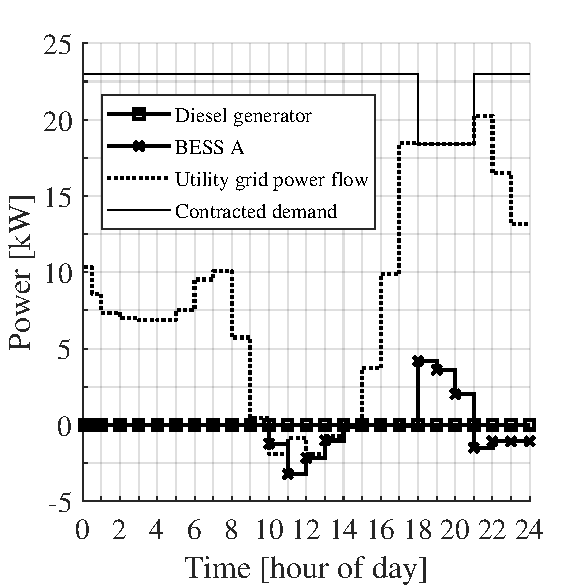
\includegraphics[width=\linewidth]{figures/residential_nv14_power.pdf}
            \caption{Power curves for scenario \ref{item:bessa+diesel}}
            \label{fig:result-power-A}
        \end{subfigure}
        \begin{subfigure}{.235\textwidth}
            \centering
            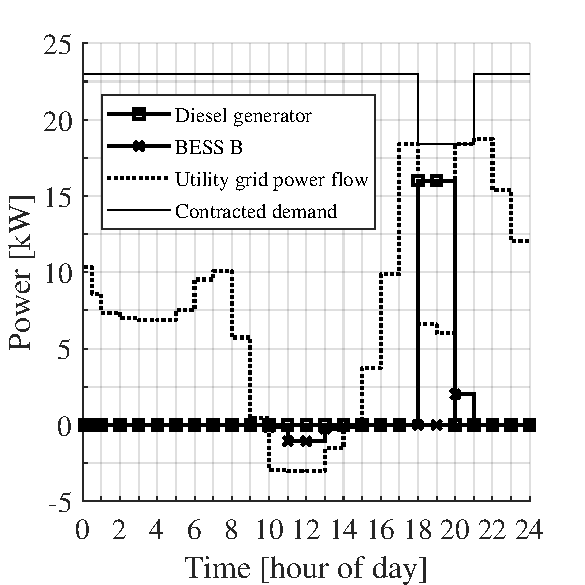
\includegraphics[width=\linewidth]{figures/residential_8ch33p_power.pdf}
            \caption{Power curves for scenario \ref{item:bessb+diesel} }
            \label{fig:result-power-B}
        \end{subfigure}

        \begin{subfigure}{.235\textwidth}
            \centering
            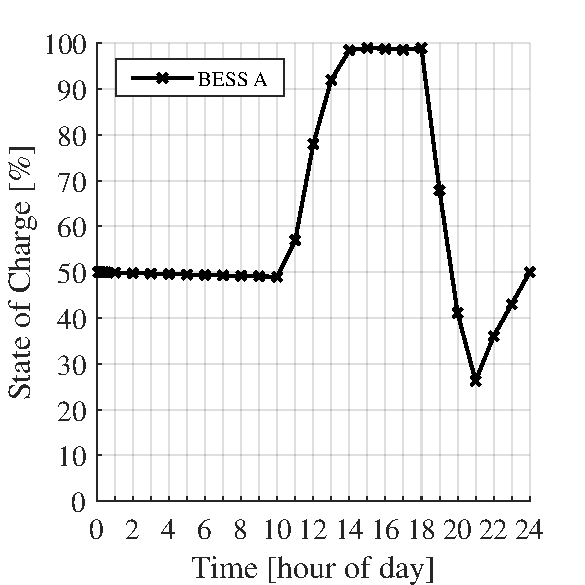
\includegraphics[width=\linewidth]{figures/residential_nv14_soc.pdf}
            \caption{Battery's SOC for scenario \ref{item:bessa+diesel}}
            \label{fig:result-soc-A}
        \end{subfigure}
        \begin{subfigure}{.235\textwidth}
            \centering
            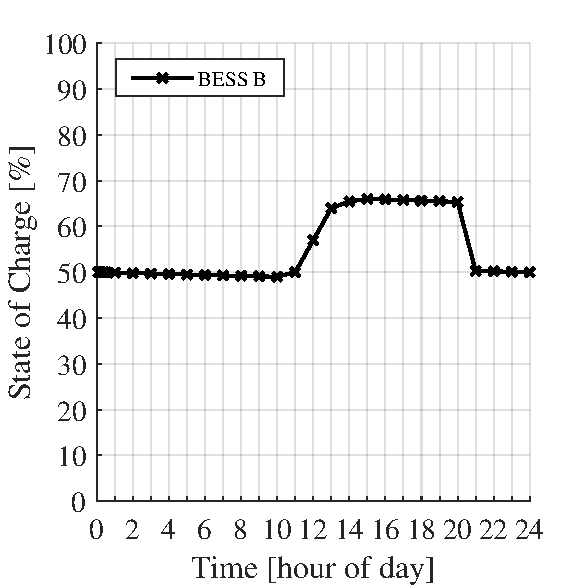
\includegraphics[width=\linewidth]{figures/residential_8ch33p_soc.pdf}
            \caption{Battery's SOC for scenario \ref{item:bessb+diesel}}
            \label{fig:result-soc-B}
        \end{subfigure}
        \caption{Results of the day-ahead planning for each battery system.}
        \label{fig:results}
    \end{figure}

    \begin{itemize}
        \item \textbf{0 a.m. -- 6 a.m.:} no PV generation, load is supplied only by the grid while, in both cases, neither BESS nor diesel generator is active. Batteries self discharge at a 0.2\% rate;
        \item \textbf{6 a.m. -- 10 a.m.:} PV generation gradually increases, until net load drops to zero;
        \item \textbf{10 a.m. -- 3 p.m.:} PV generation continues to increase, surpassing demand. Excess generation is used to charge batteries from 49.0\% to 99.0\% in scenario \ref{item:bessa+diesel} and to 66.0\% in scenario \ref{item:bessb+diesel};
        \item \textbf{3 p.m. -- 6 p.m.:} PV generation gradually decreases until zero. Batteries are kept in stand-by;
        \item \textbf{6 p.m. -- 9 p.m.:} to avoid excess demand and subsequent penalties, BESS A is cycled from 99.0\% to 26.2\% to diminish energy purchase in scenario \ref{item:bessa+diesel}, supplying roughly 10.5 kWh to the system. In contrast, in scenario \ref{item:bessb+diesel}, the diesel generator is started at 6 p.m. and stopped at 8 p.m., delivering exactly 32 kWh in two hours. This power output is more than enough to avoid excess demand and also to minimize peak-hour energy purchase --- until the quadratic consumption model limits its benefits. In the following hour, from 8 p.m. until 9 p.m., BESS B is cycled from 65.4\% to 50.3\% to supply the system.
        \item \textbf{9 p.m. -- 12 p.m.} the load curve starts to fade to a minimum whilst BESS A is recharged in scenario \ref{item:bessa+diesel} and BESS B is kept in stand-by until midnight on \ref{item:bessb+diesel}.
    \end{itemize}

    The main difference between scenarios \ref{item:bessa+diesel} and \ref{item:bessb+diesel} is notably the much deeper DOD cycle that BESS A experiences. This is due to the lower marginal cost when compared to BESS B, as can be seen in Fig. \ref{fig:wn_curves1}.

    Another interesting result is the choice of SOC range that the optimizer made for BESS A. The 10.5 kWh that it delivered represents 73\% of its capacity, and could have been cycled in either 100\%-27\% or 73\%-0\% ranges, for example. However, the 99\%-26\% indicates that the optimizer avoided the steep wear density rise near 100\% but also tried to avoid the slowly increasing wear cost near the lower end of the SOC. The same trend is observed in scenario \ref{item:bessb+diesel} but, with a much more steep rise near 100\% and overall higher wear cost, the battery is only cycled with a DOD little greater than 16\%.

    \section{Conclusion}
    Although battery wear is sometimes neglected in MG applications, it is important to incorporate a wear quantification model to avoid abusive use of the storage system. In this study we augmented the reach of a popular model by re-deriving it using a generic approach for fitting the most pervasive cycle life data that is usually made available by manufacturers. We also provided a mathematical formula that enables MG planners to evaluate and compare batteries across the entire SOC range, taking into account not only price and capacity, but also the durability of storage devices, and that could be easily customized for various batteries. The model, although simple, proved to be very useful in the implementation of an energy management algorithm that considers and minimizes battery wear, as shown by the case studies presented here, which can effectively prolong the lifespan of these devices.

    \bibliographystyle{./IEEEtran}
    \bibliography{./bibliography}

\EOD

\end{document}
